\documentclass[twocolumn]{revtex4-1}
\usepackage{amsmath}
\usepackage{mathtools}
\usepackage{xcolor}
\newcommand{\lucas}[1]{\textbf{\textcolor{blue}{LKW: #1}}}
\newcommand{\shivesh}[1]{\textbf{\textcolor{purple}{SP: #1}}}

\begin{document}
\title{A light weight regularization for wave function parameter gradients
\\ in quantum Monte Carlo}

\author{Shivesh Pathak}
\email[]{sapatha2@illinois.edu}

\author{Lucas K. Wagner}
\email[]{lkwagner@illinois.edu}
\affiliation{Department of Physics; University of Illinois at Urbana-Champaign}

\date{\today}
\begin{abstract}
The parameter derivative of the expectation value of the energy, $\partial E/\partial p$, is a key ingredient in variational quantum Monte Carlo (VMC) wave function optimization methods.
A na\"ive Monte Carlo estimate of this derivative suffers from an infinite variance which inhibits the efficiency of optimization methods that rely on a stable estimate of the derivative.
In this work, we derive a simple regularization of the na\"ive estimator which is trivial to implement in existing VMC codes, has finite variance, and a negligible bias which can be extrapolated to zero bias with no extra cost.
We use this estimator to construct an unbiased, finite variance estimation of $\partial E/\partial p$ for a multi-Slater-Jastrow trial wave function on the LiH molecule.
This regularized estimator stands as a light weight option for stable estimation of $\partial E/\partial p$ in VMC optimization techniques.
\end{abstract}
\maketitle 

\section{Introduction}
Accurate and stable stochastic estimation of the parameter gradient of the energy expectation value is an integral component of variational Monte Carlo (VMC) wave function energy optimization techniques \cite{PhysRevB.64.024512, doi:10.1063/1.1604379, Toulouse2007, Umrigar2005, Umrigar2007, Toulouse2008}.
\lucas{In general, I think you may need to build this up a little more and explain the problem.} \shivesh{tried to make it more detailed, but I think the last sentence is a bit shaky.} 
Within these techniques, the parameters $\vec{p}$ in a wavefunction $\Psi(\vec{R},\vec{p})$ are optimized to minimize the energy expectation value $E(\vec{p}) \equiv \langle \Psi(\vec{p})|\hat{H} |\Psi(\vec{p})\rangle$.
This is accomplished through iterative approaches where a stochastic estimate of the gradient $\partial E(\vec{p})/\partial p$ is used in updating the parameter $p$ at each iteration. 
If the estimate for $\partial E/\partial p$ is inaccurate, having a large bias, or unstable, having a large variance, the updates at each iteration will not be optimal, leading to inefficient wave function optimization.

The simplest estimator for $\partial E/\partial p$ is the na\"ive Monte Carlo estimate which takes the form of a covariance shown in Eqn 6 of \cite{Umrigar2005}.
This estimator is unbiased and has a zero-variance principle for any wave function parameter $p$ in the limit of $\Psi(\vec{R}, \vec{p})$ being an eigenstate of $\hat{H}$.
However, the variance of this estimator diverges when $\Psi$ is not an exact eigenstate and $p$ is a parameter which affects the nodes of the wave function, as in the case of orbital or determinantal coefficients \cite{Avella, doi:10.1063/1.4933112}.
This infinite variance problem leads to inefficient wave function optimization and has prompted a search for finite variance estimators of $\partial E/\partial p$.
\lucas{My initial impression is that this feels heavy for the introduction. We should write a simpler thing, or just save the equations for later.}
\shivesh{moved equations to later.}

Current finite variance estimation techniques were adapted from the low-variance estimation of forces in QMC \cite{doi:10.1063/1.462059, doi:10.1063/1.3516208, Phys2016} and involve guiding or auxiliary wave functions, such as a reweighting scheme \cite{Avella, Attaccalite2008, Zen2013} or improved estimators \cite{Assaraf1999, doi:10.1063/1.1286598, Assaraf2003}.
Finite variance is achieved for special guiding wave functions $\Psi_G$ which cancel the divergences present in the na\"ive Monte Carlo estimator, as discussed in the appendix of \cite{doi:10.1063/1.4933112}.
Unfortunately, using a guiding wave function within VMC will generally lead to a systematic bias in the estimate of $\partial E/\partial p$ for any finite Monte Carlo sample \cite{doi:10.1063/1.4933112, Toulouse2015}.
This bias can be reduced, but at the significant cost of evaluating variances and covariances of the MC estimator \cite{Toulouse2015} or repeating VMC calculations while tuning $\Psi_G$.
Still unresolved is an inexpensive, low-bias, low-variance estimation technique for $\partial E/\partial p$.
\lucas{"without the luggage" is not too convincing. Isn't the point that the guiding wave function doesn't need to be tuned, and that the algorithm can be simpler?}
\shivesh{language updated to be clearer about what I mean.}

We derive and test a simple regularized estimator for $\partial E/\partial p$ which has finite variance and can be efficiently extrapolated to zero bias.
Instead of relying on guiding wave functions, the divergent variance of the na\"ive Monte Carlo estimator is suppressed via multiplication by a polynomial function within a distance $\epsilon$ of the nodes of $\Psi(\vec{p}, \vec{R})$. 
We present rigorous mathematical proofs for the scalings of the variance and bias of the regularized estimator with $\epsilon$, and provide an algorithm for the zero bias extrapolation of the estimate.
The mathematical predictions and extrapolation procedure are then tested in evaluating $\partial E/\partial p$ for a multi-Slater-Jastrow (MSJ) trial wave function on the LiH molecule.

\section{Regularized estimator}
The na\"ive Monte Carlo estimate for $\partial E/\partial p$ evaluated on a wave function $\Psi(\vec{R}, \vec{p})$ is 
\begin{equation}
\hat{\theta} \equiv \left\langle \Big(E_L(\vec{R})  - \left\langle E_L(\vec{R}) \right \rangle\Big)\frac{\partial_p \Psi(\vec{R}, \vec{p})}{\Psi(\vec{R}, \vec{p})} \right\rangle
\label{eq:naive_estimator}
\end{equation} 
where the brackets $\langle \ \rangle$ are Monte Carlo expectation values over $M$ configurations drawn from the distribution $|\Psi(\vec{p}, \vec{R})|^2$, and $E_L = (\hat{H}\Psi)/\Psi$ is the local energy with Hamiltonian operator $\hat{H}$.
This estimator has zero bias for any wave function $\Psi$ and parameter $p$, but can acquire a divergent variance.
\lucas{Should explain the na\"ive estimator here in a little more detail.}
\shivesh{Moved it.}
The divergent contribution to the variance arises from the evaluation of the integral
\begin{equation}
\int \Big(E_L\frac{\partial_p\Psi}{\Psi}\Big)^2 |\Psi|^2 dR.
\label{eq:divergent_integral}
\end{equation}
when $\Psi$ is not an eigenstate of $\hat{H}$ and the parameter $p$ affects the nodes of $\Psi$, such as orbital or determinantal coefficients.
In this case, to lowest order in distance $|\vec{R}-\vec{N}|$ from a nodal point $\vec{N}$ of $\Psi$, $\hat{H}\Psi$ and $\partial_p \Psi \sim const$ and $\Psi \sim \nabla \Psi(\vec{N}) \cdot (\vec{R} - \vec{N})$, leading to the integrand in Eqn~\ref{eq:divergent_integral} behaving as $1/|\vec{R}-\vec{N}|^2$ near the node.
Since the integration domain includes the nodal surface of $\Psi$, the $1/|\vec{R}-\vec{N}|^2$ behavior of the integrand as $|\vec{R}-\vec{N}|\rightarrow 0$ leads to a divergent integral.

We obtain a finite variance estimator for $\partial E/\partial p$ by regularizing the na\"ive estimator of Eqn~\ref{eq:naive_estimator} by a function $f_\epsilon$:
\begin{equation}
\hat{\theta} \equiv \left\langle \Big(E_L(\vec{R})  - \left\langle E_L(\vec{R}) \right \rangle\Big)\frac{\partial_p \Psi(\vec{R}, \vec{p})}{\Psi(\vec{R}, \vec{p})} f_\epsilon(\vec{R}) \right\rangle
\label{eq:regularized_estimator}
\end{equation}
\lucas{the notation with all the summations is not very easy to read to me. Typically we would say something like $\left\langle E_L(R) \frac{\partial_p \Psi(R)}{\Psi(R)} f_\epsilon(R) \right\rangle_{R\sim\Psi_T^2}$. Also, is the second expectation value also regularlized? Why not?}
\shivesh{Updated the summations. The second term does need to be regularized, added that in}.
where 
\begin{equation}
\begin{split}
&f_\epsilon(\vec{R}) = \begin{cases} 
     7(\frac{\vec{x}}{\epsilon})^6 - 15(\frac{\vec{x}}{\epsilon})^4 + 9(\frac{\vec{x}}{\epsilon})^2 & |\frac{\vec{x}}{\epsilon}| < 1 \\
      1 & |\frac{\vec{x}}{\epsilon}| \ge 1 \\
   \end{cases}\\ 
 &\vec{x} \equiv \frac{\nabla \Psi(\vec{R}) \Psi(\vec{R})}{|\nabla \Psi(\vec{R})|^2}.
\end{split}
\label{eq:regularizing_function}
\end{equation} 
\lucas{What does the O notation mean here? This is not explained? If it's meant to be big-O notation, that uses $\mathcal{O}$, and it shouldn't be used here. Just say that it's proportional to.} 
\shivesh{Updated to remove any O and just explicitly write down the general form of $f_\epsilon$.}
Details on the construction of $f_\epsilon$ can be found in the Appendix.

The regularized estimator in Eqn~\ref{eq:regularized_estimator} achieves a finite variance by replacing the previously divergent integral Eqn~\ref{eq:divergent_integral} with a finite one
\begin{equation}
\begin{split}
\int \Big(E_L\frac{\partial_p\Psi}{\Psi}\Big)^2 f_\epsilon^2 |\Psi|^2 dR = \int_{|x/\epsilon|\geq 1} \Big(E_L\frac{\partial_p\Psi}{\Psi}\Big)^2 |\Psi|^2 dR +\\ \int_{|x/\epsilon|< 1} \Big(E_L\frac{\partial_p\Psi}{\Psi}\Big)^2 f_\epsilon^2 |\Psi|^2 dR.
\end{split}
\label{eq:convergent_integral}
\end{equation}
This is readily verified by breaking up the integral into two domains as shown above.
Since $\Psi = 0$ only occurs when $\vec{x} = 0$, the integral for $|\vec{x}/\epsilon|\geq 1$ completely excludes the nodal surface of $\Psi$, and is finite. 
Further, since $|\vec{x}/\epsilon| \sim |\nabla\Psi(\vec{N}) \cdot (\vec{R}-\vec{N})|/\epsilon|\nabla  \Psi(\vec{N})|$ as $|\vec{R} - \vec{N}| \rightarrow 0$, the integrand arbitrarily close to the nodal surface is $\propto |\vec{R} - \vec{N}|^2$, meaning the second integral for $|\vec{x}/\epsilon| < 1$ is also finite.

\lucas{It looks like the following attempts to show how one figures out the correct form form $f_\epsilon$. This is good for a talk (or an appendix!), but bad for a paper. You're trying to establish that a given estimator has low bias and variance, not show how to construct it. }
\shivesh{Moved construction to appendix.}
Not only is the variance finite, but the variance of Eqn~\ref{eq:regularized_estimator} decreases exponentially as $1/\epsilon$ to lowest order in $\epsilon$.
This is a consequence of $f_\epsilon$ being dimensionless, which ensures that all contributions to the $|\vec{x}/\epsilon|< 1$ integral in Eqn~\ref{eq:convergent_integral} take the form:
\begin{equation}
\int_{|\vec{x}/\epsilon|< 1} \Big(E_L\frac{\partial_p\Psi}{\Psi}\Big)^2 |\frac{\vec{x}}{\epsilon}|^{2n} |\Psi|^2 dR
\end{equation} 
where $n \geq 1$ is an integer.
\lucas{What does non-dimensionality mean?} \shivesh{Meant to say dimensionless.}
As $\epsilon \rightarrow 0$, the integration domain is very near the nodal surface and the integrand can be Taylor expanded to lowest order in $|\vec{R}-\vec{N}|$. 
The Taylor expansion yields an integrand $|\vec{x}/\epsilon|^{n-2}/\epsilon^2$ and results in an integral which scales as $O(1/\epsilon)$ to lowest order in $\epsilon$.

The exponentially suppressed variance of the estimate comes at a cost, in the form of cubic bias $O(\epsilon^3)$ to lowest order in $\epsilon$.
The bias of the regularized estimator is
\begin{equation}
\text{Bias: } \int_{|\vec{x}/\epsilon|< 1} H\Psi \partial_p \Psi (f_\epsilon - 1) dR.
\label{eq:estimator_bias}
\end{equation}
Following the analysis of the previous paragraph, we evaluate the bias to lowest non-vanishing order in $\epsilon$ by Taylor expanding $H\Psi \partial_p\Psi$ in powers of $|\vec{R} - \vec{N}|$ and calculating the bias at each order in the expansion.
The constant and linear order terms in the Taylor expansion do not contribute to the bias, the latter by parity of the integrand, the prior by explicit integration of $f_\epsilon$ in Eqn~\ref{eq:regularizing_function}.
The lowest non-vanishing contribution to the bias is due to term in the Taylor expansion $\propto |\vec{R} - \vec{N}|^2$, yielding an integral which scales as $\epsilon^3$.

This cubic bias can be removed by a zero-bias extrapolation carried out in four steps.
\begin{enumerate}
\item Conduct a standard VMC calculation to collect $M$ configurations from $|\Psi|^2$.
\item Evaluate $|\vec{x}_i|$ from Eqn~\ref{eq:regularizing_function} for each configuration.
\item Calculate the regularized estimate Eqn~\ref{eq:regularized_estimator} for a sequence of $\epsilon \rightarrow 0$ on the collected configurations.
\item Fit a function $a\epsilon^3 + b$ to the estimates; the intercept $b$ is the zero bias, finite variance estimate for $\partial E/\partial p$.
\end{enumerate}
This procedure can be carried out very efficiently as only a single set of VMC configurations must be drawn for the entire extrapolation, resulting in an inexpensive, finite-variance, zero bias estimate of $\partial E/\partial p$.

\lucas{If it's an enumerated list, just make it one; it's easier to read than text. This phrasing is a little weird because it makes it sound more complicated. Aren't you just taking the expectation value as a function of $\epsilon$ and extrapolating to zero?} 
\shivesh{Updated to an enumerated list.}

\section{Application to LiH molecule}
We verify the predicted mathematical behavior of $\hat{\theta}_\epsilon$ by using it to estimate $\partial E/\partial p$ for a determinantal coefficient of a MSJ wave function for the LiH molecule
\begin{equation}
\Psi(\vec{c}, \vec{\alpha}) = e^{J(\vec{\alpha})} \sum_{i} c_i  |D_i \rangle.
\end{equation}
The determinants $|D_i \rangle$ and coefficients $c_i$ were taken from a full configuration interaction (CI) expansion over the Li 1s, 2s, 2p and H 1s orbitals.
The orbitals were constructed from a restricted open-shell Hartree Fock (ROHF) calculation using a correlation consistent quadruple-zeta valence basis set \cite{doi:10.1063/1.456153}.
A 2-body Jastrow factor $J(\vec{\alpha})$ of the form in \cite{Wagner2009} was used with $\vec{\alpha} = 0$ except for appropriate electron-electron cusp conditions.
The parameters $\vec{\alpha}, \vec{c}$ were not optimized further in order to emulate a trial function to be used in a standard VMC energy optimization calculation.
\lucas{This seems to imply that you did not optimize the Jastrow. You should just write out the wave function ansatz and indicate what parameters were optimized.}
\shivesh{Wrote out wave function ansatz and what parameters were optimized. I did not optimize the Jastrow, see the explanation in the added last sentence. I can optimize it and run the figure calculations again if needed, no problem.}
The ROHF and CI calculations were done using the PySCF package \cite{PYSCF} and all QMC calculations were carried out using PyQMC \cite{pyqmc}.

\begin{figure}
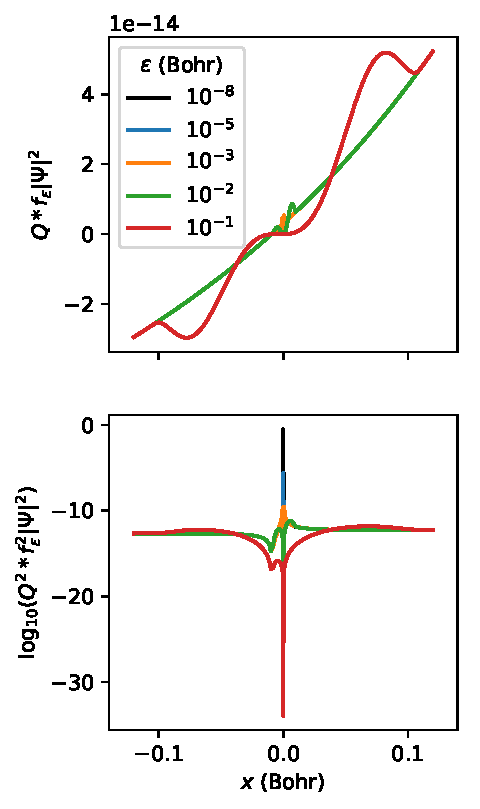
\includegraphics[width=1.0\columnwidth]{../2_plots/viznode.pdf}
\caption{$E_L\frac{\partial_p \Psi}{\Psi} f_\epsilon$ and logarithm $(E_L\frac{\partial_p \Psi}{\Psi} f_\epsilon)^2$, plotted against the normal coordinate $x$ from a node of $\Psi$. Curve colors correspond to different values of $\epsilon$ ranging from $10^{-1}$ to $10^{-8}$ Bohr.}
\end{figure}

\begin{figure}
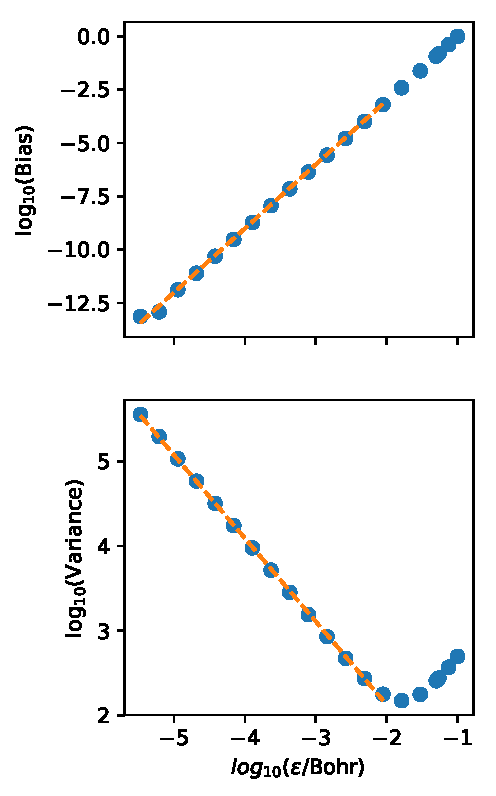
\includegraphics{../2_plots/integratenode.pdf}
\caption{Scaled bias and variance of $E_L\frac{\partial_p \Psi}{\Psi}$ evaluated by numerical integration from $r = -0.1$ to $r = 0.1$ across the node in Figure 1. The blue dots are the numerically integrated values and the orange curves indicate best fits to the functions $a\epsilon^3$ and $b + c/\epsilon$ for the bias and variance, respectively.}
\end{figure}

\begin{figure}
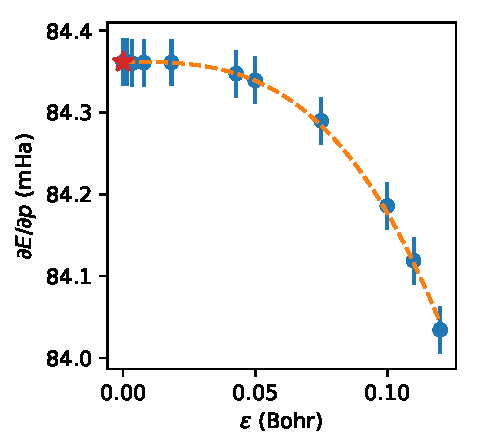
\includegraphics{../2_plots/dedp.pdf}
\caption{Zero bias, finite variance extrapolation for $\partial E/\partial p$ using the regularized estimator. The blue points are evaluated using VMC, the orange curve is a fit to $a + b\epsilon^3$, and the red star denotes the extrapolated estimation. }
\end{figure}

We begin by verifying that the regularized integral in Eqn~\ref{eq:convergent_integral} has finite value for $\epsilon > 0$. \lucas{The integrand is not making a claim. Be more specific. Are we just verifying Eqn \ref{eq:convergent_integral}?}
\shivesh{Updated to be more specific.}
To do so, we evaluate the regularized integrand for various $\epsilon$ along a path which passes through a node $\vec{N}$, $\vec{R}(x) = \vec{N} + x \nabla \Psi(\vec{N})/|\nabla \Psi(\vec{N})|$ with $x \in [-0.1, 0.1]$ Bohr.
The results are shown in the lower plot of Figure 1.
For all values of $\epsilon$, the value of the integrand is pushed to zero at the node, removing the divergence in the integral.
The sharp increase in the integrand near $x=0$ as $\epsilon$ decreases is indicative of the increase in the value of the integral, and hence estimator variance, as $\epsilon \rightarrow 0$.
Shown in the upper plot is the first term in Eqn~\ref{eq:regularized_estimator} across the node, exhibiting no divergences.

By integrating across the normal coordinate $x$, the predicted $O(1/\epsilon)$, $O(\epsilon^3)$ scalings of the variance and bias are recovered, as shown in Figure 2.
The integration for both the bias and variance are carried out for the path in Figure 1 from $x = -0.1$ to $0.1$ Bohr and normalized by a factor $\int |\Psi|^2 dR$ along that path.
The predicted cubic bias is observed for six decades in $\epsilon$ while the exponential decrease in variance stands for four decades.
The increase in the variance after $\epsilon = 10^{-2}$ occurs due to the breakdown of the assumption $\Psi(\vec{R}) \sim \nabla(\vec{N}) \cdot (\vec{R}-\vec{N})$, resulting in a linear increase in variance with $\epsilon$.
This change is not mirrored in the bias since the sub-leading order scaling with $\epsilon$ appears when the assumptions of $\hat{H}\Psi$ and $\partial_p \Psi \sim const$ break down.

We conclude by carrying out the four step, zero-bias, finite variance extrapolation for $\partial E/\partial p$ proposed in the previous section, shown in Figure 3.
First, a standard VMC calculation with 200,000 steps and 2,000 configurations per step was carried out.
Then, $\partial E/\partial p$ was estimated using Eqn~\ref{eq:regularized_estimator} for $\epsilon$ between $10^{-1}$ Bohr and $10^{-5}$ Bohr using the VMC configurations, shown in the blue data points.
Since the same configurations were used for each evaluation, the estimates have a strong statistical correlation and the predicted $\epsilon^3$ bias is clearly present, shown by the orange fit curve.
The intercept of the fit curve is shown by the red star and is the zero-bias estimate of $\partial E/\partial p$.
The variance can be deduced by the error bar of the blue data points, in this case 0.025 mHa.
Since the bias is zero within statistical errors for small values of $\epsilon$, most practical calculations can be carried out for a fixed value of $\epsilon$ between $10^{-5}$ and $10^{-2}$ Bohr without extrapolation.
Thus the regularized estimator is quite robust to $\epsilon$.

\section{Conclusion}
In this work, we derived and tested a simple regularized estimator for $\partial E/\partial p$ which has finite variance and can be extrapolated to zero bias.
The divergent variance present in the na\"ive Monte Carlo estimator is suppressed via multiplication by a polynomial function within a distance $\epsilon$ of the nodes of $\Psi(\vec{p}, \vec{R})$. 
We prove that the regularized estimator manages a finite variance by incurring a cubic bias which can be efficiently extrapolated to zero bias.
The extrapolation is carried out, and a finite variance, zero-bias estimate of $\partial E/\partial p$ is evaluated for a determinantal coefficient in a trial wave function for the LiH molecule.

The regularized estimator stands as an improvement to popular guiding wave function techniques \cite{Avella, Attaccalite2008, Zen2013, Assaraf1999, doi:10.1063/1.1286598, Assaraf2003} for the low-bias, low-variance estimation of $\partial E/\partial p$.
In the latter, finite variance is achieved by using a guiding wave function to sample Monte Carlo configurations.
The finite variance comes at the cost of a systematic bias which must be corrected with significant computational expense either by tuning the guiding wave function or evaluating covariances of the estimator \cite{ Toulouse2015}.
The regularized estimator also has finite variance and non-zero bias for any $\epsilon > 0$, but no additional cost is incurred in extrapolating the estimate to zero bias.
As such, the regularized estimator is an efficient option for the accurate and stable estimation of $\partial E/\partial p$ in VMC optimization techniques.

\lucas{explain why this is advantageous and an improvement of the state of the art. }
\shivesh{removed "intro"-ish paragraph, added a second one talking about advantages.}

%\bibliographystyle{unsrt}
\bibliography{pgradregr}

\section{Appendix}
The following are details on the construction of $f_\epsilon$ seen in Eqn~\ref{eq:regularizing_function}. 
We begin with the general form of a regularized estimator
$$
\hat{\theta_\epsilon} \equiv
\left\langle E_L(R) \frac{\partial_p \Psi(R)}{\Psi(R)} f_\epsilon(R) \right\rangle - \left\langle E_L(R) \right \rangle \left \langle \frac{\partial_p \Psi(R)}{\Psi(R)} f_\epsilon(R) \right\rangle
$$
where 
\begin{equation}
f_\epsilon(\vec{R}) = \begin{cases} 
      \sum_{n=1}^{\infty} a_n |\frac{\vec{x}}{\epsilon}|^n & |\frac{\vec{x}}{\epsilon}| < 1 \\
      1 & |\frac{\vec{x}}{\epsilon}| \ge 1 \\
   \end{cases},\ \vec{x} \equiv \frac{\nabla \Psi(\vec{R}) \Psi(\vec{R})}{|\nabla \Psi(\vec{R})|^2}.
\end{equation} 

The previously divergent contribution to the estimator variance Eqn~\ref{eq:divergent_integral} is replaced by a finite integral, verified by piecewise integration
$$
\int \Big(E_L\frac{\partial_p\Psi}{\Psi}\Big)^2 f_\epsilon^2 |\Psi|^2 dR = $$
$$ \int_{|x/\epsilon|\geq 1} \Big(E_L\frac{\partial_p\Psi}{\Psi}\Big)^2 |\Psi|^2 dR +\\ \int_{|x/\epsilon|< 1} \Big(E_L\frac{\partial_p\Psi}{\Psi}\Big)^2 f_\epsilon^2 |\Psi|^2 dR,
$$
Since $\Psi = 0$ only occurs when $\vec{x} = 0$, the integral for $|\vec{x}/\epsilon|\geq 1$ completely excludes the nodal surface of $\Psi$, and is finite. 
Further, since $|\vec{x}/\epsilon| \sim |\nabla\Psi(\vec{N}) \cdot (\vec{R}-\vec{N})|/\epsilon|\nabla  \Psi(\vec{N})|$ as $|\vec{R} - \vec{N}| \rightarrow 0$, the integrand arbitrarily close to the nodal surface is a constant, meaning the second integral for $|\vec{x}/\epsilon| < 1$ is also finite.

Unfortunately, the regularized estimator results in a linear-order biased estimation of $\partial E/\partial p$.
The bias results only from the first term and is written as 
$$
\text{Bias: } \int_{|\vec{x}/\epsilon|< 1} \Big(E_L\frac{\partial_p\Psi}{\Psi}\Big) (f_\epsilon - 1)|\Psi|^2 dR.
$$
As before, we take $\epsilon \rightarrow 0$ and Taylor expand the integrand to lowest order in $|\vec{R}-\vec{N}|$.
This yields an integrand, to lowest order in $\epsilon$, $a_1|\vec{x}/\epsilon| - 1$.
Carrying out the integration yields a bias that scales as $O(\epsilon)$ to lowest order in $\epsilon$.
The linear bias is inhibitive to zero bias extrapolation as the estimation bias is present for any value of $\epsilon$ while the variance increases exponentially with $\epsilon \rightarrow 0$.

A simple normalization condition on $f_\epsilon$ ensures a bias of $O(\epsilon^3)$, allowing for efficient extrapolation to zero bias.
The expression for the bias as $\epsilon \rightarrow 0$ after carrying out the necessary Taylor expansions is
$$
\lim_{\epsilon\rightarrow 0}\text{Bias} =  A \int_{|\vec{x}/\epsilon|< 1} (f_\epsilon - 1) dR.
$$
where $A$ is a constant resulting from $\hat{H}\Psi$ and $\partial_p \Psi \sim const$ as $|\vec{R}-\vec{N}|\rightarrow 0$.
As such, the linear order bias can be removed by enforcing a normalization condition on $f_\epsilon$ on the domain of integration, 
$$
\int_{|\vec{x}/\epsilon|< 1} (f_\epsilon - 1) dR = 0.
$$
The leading order contribution to the bias arises from the breakdown of the Taylor approximation $\hat{H}\Psi$ and $\partial_p \Psi \sim const$, and results in a bias $O(\epsilon^3)$.
The quadratic contribution to the bias is zero as $f_\epsilon$ is even in $|\vec{R}-\vec{N}|$.

A final set of continuity and smoothness conditions on $f_\epsilon$ at $|\vec{x}/\epsilon| = 1$ reduce the magnitude of the cubic bias.
These two conditions can be written as 
$$
f(1) = 1, \nabla f(1) = 0.
$$
The three conditions, smoothness, continuity and normalization, can all be satisfied with a polynomial formula for $f$
$$
f_\epsilon(|\frac{\vec{x}}{\epsilon}|) = 7(\frac{\vec{x}}{\epsilon})^6 - 15(\frac{\vec{x}}{\epsilon})^4 + 9(\frac{\vec{x}}{\epsilon})^2.
$$

\end{document}
